\chapter{Elaborazione dei dataset (ETL)} \label{chap:elaborazione}

	Nello sviluppo di questa progetto sono stati usati i \textit{dataset} contenenti il bilancio del 2012 e del 2013 del Comune di Firenze, reperibili sul sito degli \textit{opendata} di Firenze\footnote{\url{http://opendata.comune.fi.it/}}.\\
	Questi \textit{dataset} contengono i dati principali delle fatture dei fornitori del Comune di Firenze per le quali, nel periodo che va dal 26 giugno 2012 (data di entrata in vigore di quanto disposto dall'art.18 del Decreto Sviluppo 2012) fino al 17 dicembre  2012, sono stati sia emessi che quietanzati i mandati di pagamento. Sempre con riferimento a tale articolo, sono stati selezionati gli elementi informativi pubblicati per ciascuna fattura.\\
	\\
	Per quanto riguarda la struttura dei \textit{dataset} essi sono strutturati allo stesso modo, con l'unica eccezione per il bilancio del 2012, che possiede un campo aggiuntivo identificante il numero di mandato (\texttt{NUMERO\_MANDATO}).\\
	Escluso l'eccezione appena introdotta la struttura generale è la seguente:
	\begin{itemize}
		\item \texttt{BENEFICIARIO}: Azienda o privato a cui è stato commissionato un mandato;
		\item \texttt{PARTITA\_IVA\_O\_CF}: partita iva o codice fiscale del beneficiario;
		\item \texttt{IMPORTO}: importo pagato (o ricevuto) dal Comune;
		\item \texttt{ATTO\_DI\_IMPEGNO}: codice contenente il tipo, il numero e l'anno di stipula dell'atto d'impegno;
		\item \texttt{DIREZIONE\_SERVIZIO\_RESP\_PROC}: Direzione di Servizio del Comune di Firenze che ha commissionato il lavoro;
		\item \texttt{DOCUMENTO}: il tipo di documento (fattura/nota di credito).
	\end{itemize}
	
	Lo scopo di questo lavoro è integrare tra loro i \textit{dataset} relativi ai bilanci annuali in modo da poter compiere successivamente delle analisi che non siano ristrette ad un singolo anno, ma che possano confrontare anche i dati su più anni di bilancio. Permetteremo così anche un'analisi temporale dei flussi di pagamento e di credito del Comune di Firenze. Ad esempio cercheremo di integrare i dati in modo tale da permettere il recupero di informazioni come la lista delle aziende a cui sono stati commissionati lavori più lunghi o come variano gli investimenti nei vari settori del Comune di Firenze tra il 2012 ed il 2013.\\
	\\
	Lo strumento utilizzato in questa prima fase è \textit{Kettle}: \textit{Kettle} è un tool di \textit{Data Integration} che permette di specificare, a partire dalle sorgenti dati, una serie di operazioni che produrranno i dati aggregati (o derivati) in output. Sia gli input che gli output possono essere tabelle di Database vere e proprie, oppure, come nel nostro caso, un file \texttt{.csv}, che costituisce un insieme di dati tra loro anche ridondanti.\\
	
	\section{Trasformazione} \label{sec:trasformazione}
		
		Vedremo adesso nel dettaglio la trasformazione \textit{Kettle} che è stata costruita ed utilizzata per questo progetto.
		
		
		\begin{figure}[h!]
			\centering
				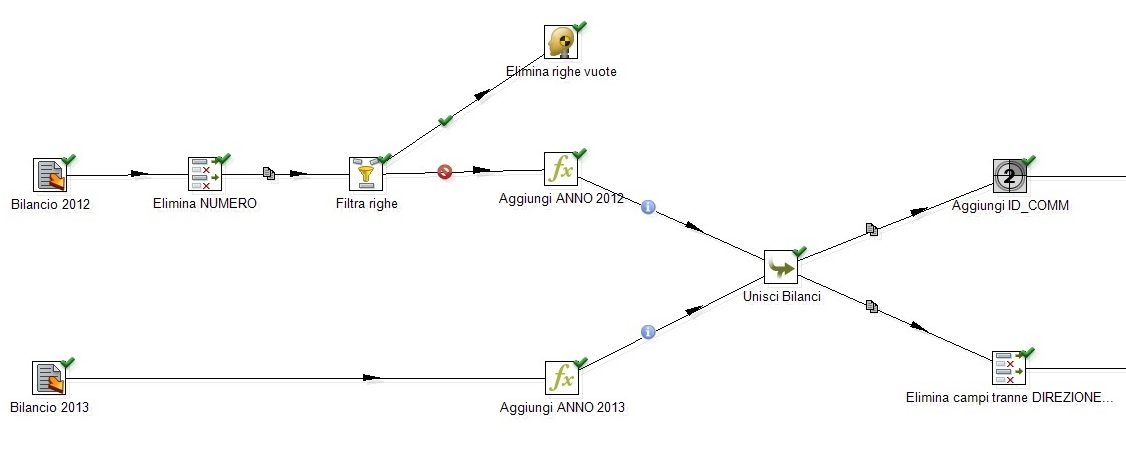
\includegraphics[scale=0.4]{transf1.jpg}
			\caption{Trasformazione Kettle, prima parte.}
			\label{fig:transf1}
		\end{figure}
		
		In questa prima parte della trasformazione (Figura \ref{fig:transf1}) si provvede innanzitutto a caricare le sorgenti dati dell'algoritmo collegate ai file dei vari \textit{dataset} da integrare. Quindi si riportano i due \textit{dataset} ad una struttura comune, eliminando dal bilancio 2012 il campo superfluo \texttt{NUMERO\_MANDATO}, eliminando le eventuali righe vuote ed aggiungendo a ciascun bilancio il relativo anno di appartenenza (campo \texttt{ANNO\_PAGAMENTO}). Infine i due flussi d'input vengono concatenati (funzione di \textit{append}) l'uno di seguito all'altro. Si osservi che in questo caso, come per il resto della trasformazione, l'ordine di concatenazione dei vari flussi è indifferente, in quanto tra gli ultimi step della trasformazione verrà eseguito un ordinamento.\\
		
		\begin{figure}[h!]
			\centering
				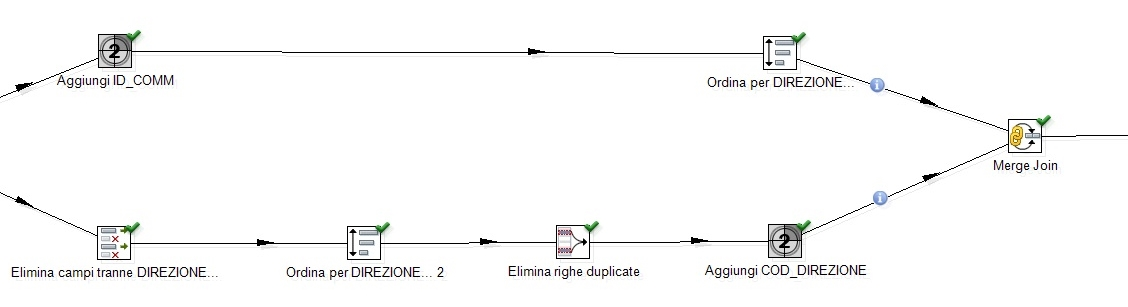
\includegraphics[scale=0.4]{transf2.jpg}
			\caption{Trasformazione Kettle, seconda parte.}
			\label{fig:transf2}
		\end{figure}
		
		A partire dall'unico elenco di commissioni precedentemente generato si generano due flussi di esecuzione (Figura \ref{fig:transf2}): nel primo si provvede ad aggiungere un identificativo per ogni commissione (ovvero per ogni riga presente), chiamato \texttt{ID\_COMM}, e successivamente ad ordinare il tutto rispetto alla direzione di servizio (vincolo necessario per eseguire un merge-join); nel secondo flusso generato, invece, si considerano le sole direzioni di servizio, eliminando ogni altro campo, ed eliminando le voci duplicate (quindi mantenendo una riga per ogni direzione distinta), per poter poi aggiungere un identificativo (\texttt{COD\_DIREZIONE}) ad ognuna di esse. Infine tramite l'utilizzo di un merge-join si provvede ad unire (e non concatenare, come nel caso precedente) i due flussi, così da avere al termine di questi passi per ogni commissione un proprio identificativo e oltre al campo con il nome della direzione di servizio sarà presente anche il codice corrispettivo.\\
		
		\begin{figure}[h!]
			\centering
				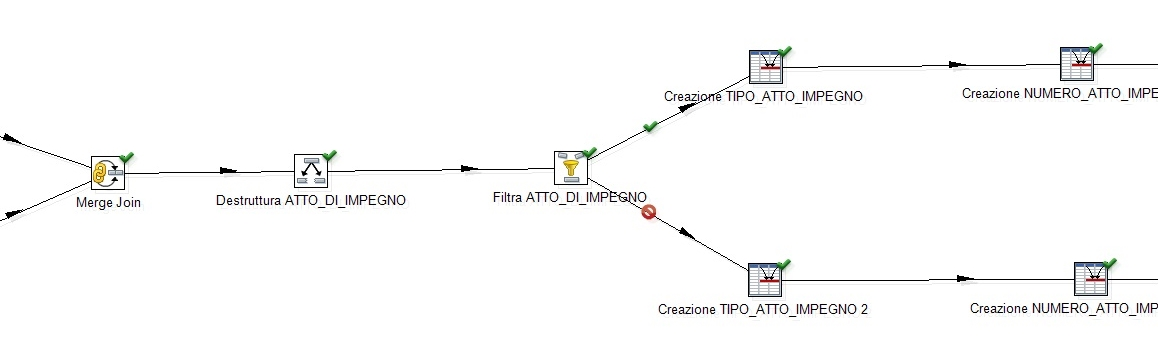
\includegraphics[scale=0.4]{transf3.jpg}
			\caption{Trasformazione Kettle, terza parte.}
			\label{fig:transf3}
		\end{figure}
		
		\begin{figure}[h!]
			\centering
				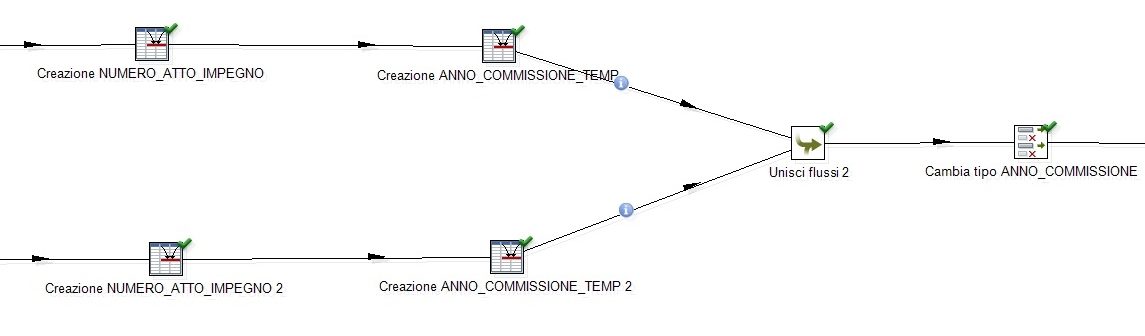
\includegraphics[scale=0.4]{transf4.jpg}
			\caption{Trasformazione Kettle, quarta parte.}
			\label{fig:transf4}
		\end{figure}
		
		I passi presenti nelle Figure \ref{fig:transf3} e \ref{fig:transf4} hanno come obiettivo quello di destrutturare il campo \texttt{ATTO\_DI\_IMPEGNO}, nel quale è tenuto traccia dell'anno di commissione del lavoro, che risulterà utile in fase di analisi. Come si può intuire osservando le figure, l'atto d'impegno è destrutturato nei campi:
		\begin{itemize}
			\item \texttt{TIPO\_ATTO\_IMPEGNO}: suddiviso essenzialmente in \textit{CC} (Consiglio Comunale) e \textit{DD} (Decreto, o Determina, Dirigenziale), indica a che livello è stata deliberata la commissione;
			\item \texttt{NUMERO\_ATTO\_IMPEGNO}: identifica univocamente gli atti d'impegno (si osservi che più commissioni possono riferirsi allo stesso atto d'impegno);
			\item \texttt{ANNO\_DI\_COMMISSIONE\_TEMP}: campo temporaneo in cui vengono registrate le ultime due cifre dell'anno di commissione.
		\end{itemize}
		Al termine di questi passi di destrutturazione vengono riuniti i flussi e viene associato un tipo intero al campo \texttt{ANNO\_DI\_COMMISSIONE\_TEMP}.\\
		
		\begin{figure}[h!]
			\centering
				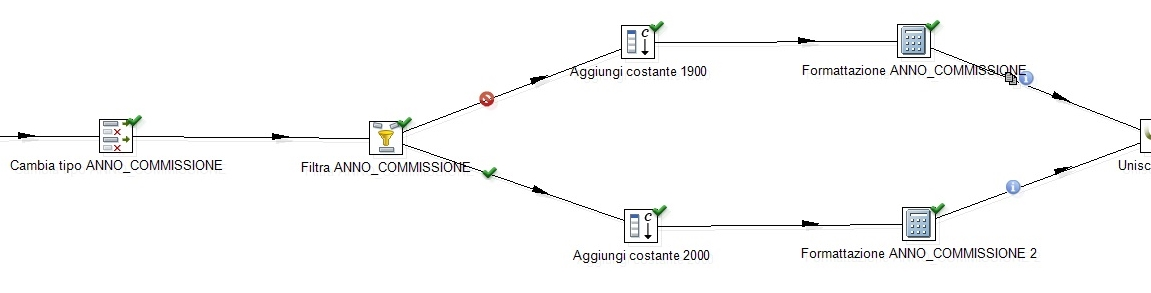
\includegraphics[scale=0.4]{transf5.jpg}
			\caption{Trasformazione Kettle, quinta parte.}
			\label{fig:transf5}
		\end{figure}
		
		I passi rappresentati nella Figura \ref{fig:transf5} hanno invece come obiettivo quello di formattare nel modo corretto l'anno di commissione estratto dall'atto d'impegno: si provvede innanzitutto a discriminare, tramite un filtro, che l'anno sia relativo al 1900 o al 2000 (alcuni atti d'impegno risalgono a più di vent'anni fa!); quindi si generano due flussi di esecuzione, che provvedono ad aggiungere le costanti 1900 o 2000 al campo \texttt{ANNO\_DI\_COMMISSIONE\_TEMP}, generando il nuovo campo \texttt{ANNO\_DI\_COMMISSIONE}; infine si provvede a riunire due flussi.
		
		\begin{figure}[h!]
			\centering
				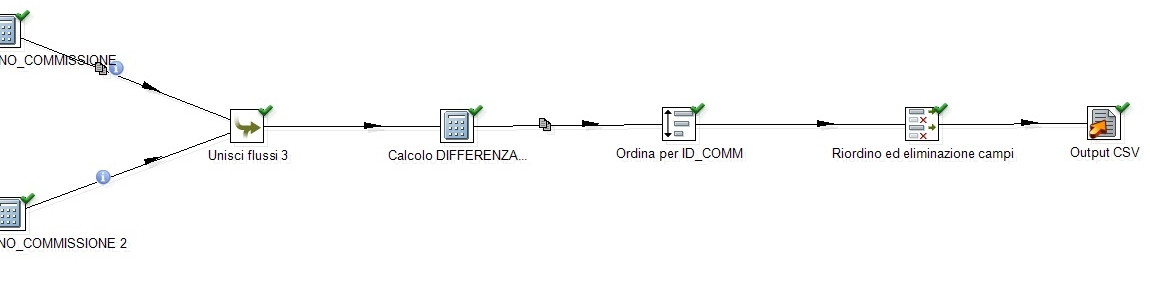
\includegraphics[scale=0.4]{transf6.jpg}
			\caption{Trasformazione Kettle, sesta parte.}
			\label{fig:transf6}
		\end{figure}
		
		Gli ultimi passi della trasformazione (rappresentati in Figura \ref{fig:transf6}) hanno come obiettivo quello di aggiungere un campo derivato, anch'esso necessario in fase d'analisi. Il campo in questione è \texttt{DIFFERENZA\_PAGAMENTO\_COMMISSIONE}, calcolato come differenza tra l'anno di pagamento (associato al bilancio stesso) e l'anno di commissione (precedentemente estratto dall'atto d'impegno).\\
		Le ultime operazioni provvedono ad ordinare tutte le commissioni, ad eliminare i campi non necessari all'analisi e riordinare tra loro quelli utili.\\
		Infine viene generato l'output della trasformazione, \texttt{Commissioni.csv}, che contine tutte le commissioni registrate nei due anni e presenta in quest'ordine i seguenti campi:
		\begin{itemize}
			\item \texttt{ID\_COMM}
			\item \texttt{PARTITA\_IVA\_O\_CF}
			\item \texttt{BENEFICIARIO}
			\item \texttt{COD\_DIREZIONE}
			\item \texttt{DIREZIONE\_SERVIZIO\_RESP\_PROC}
			\item \texttt{IMPORTO}
			\item \texttt{DOCUMENTO}
			\item \texttt{TIPO\_ATTO\_IMPEGNO}
			\item \texttt{NUMERO\_ATTO\_IMPEGNO}
			\item \texttt{ANNO\_COMMISSIONE}
			\item \texttt{ANNO\_PAGAMENTO}
			\item \texttt{DIFFERENZA\_PAGAMENTO\_COMMISSIONE}
		\end{itemize}
		
		
	\section{Job}\label{sec:job}
		La trasformazione presentata nella sezione precedente è quella che sta alla base del \textit{job} che verrà poi eseguito anno per anno per integrare i nuovi \textit{dataset} ai precedenti.\\
		In generale, infatti, ogni volta che verrà rilasciato un nuovo \textit{dataset} sarà necessario appendere al file \texttt{.csv}, contenente i dati aggregati dei bilanci precedenti, il nuovo bilancio opportunamente modificato, per avere una struttura coerente con le precedenti.\\
		Il \textit{job} di trasformazione è il seguente:\\
		
		\begin{figure}[h!]
			\centering
				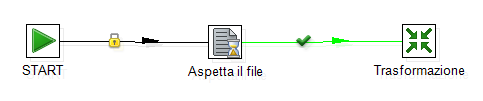
\includegraphics[scale=1]{job.png}
			\caption{\textit{Job} di trasformazione.}
			\label{fig:job}
		\end{figure}
		
		\begin{figure}[h!]
			\centering
				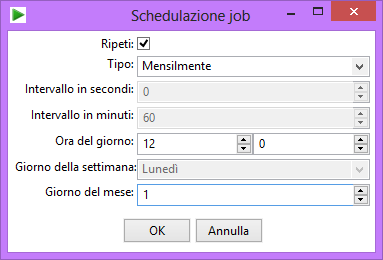
\includegraphics[scale=0.7]{job_scheduling.png}
			\caption{Impostazioni di scheduling del job.}
			\label{fig:job_scheduling}
		\end{figure}
		
		Dalla Figura \ref{fig:job} deduciamo subito la semplicità del \textit{job}: esso è formato da uno step \textit{start}, che definisce il punto di inizio e le impostazioni di scheduling, uno step di attesa, che blocca il flusso finché non è presente il \texttt{.csv} del nuovo bilancio da integrare, ed uno step \textit{trasformazione}, che è esattamente la trasformazione \textit{Kettle} precedentemente descritta in questo capitolo, opportunamente rivista per gestire un qualsiasi file di bilancio. Nella Figura \ref{fig:job_scheduling} vediamo invece il dettaglio dello step \textit{start}, dove vengono definite le impostazioni di scheduling, in modo da eseguire l'integrazione dei nuovi dati ad intervalli prefissati ed in modo del tutto automatico.\\
		\\
		In questa sezione abbiamo descritto come produrre una sorgente dati singola, dettagliata, esauriente e di alta qualità che possa alimentare il DW a partire da dati operazionali reperiti all'interno di \textit{dataset}.\\
		Le operazioni svolte, o che è possibile svolgere, tramite \textit{Kettle} sono estrazione, pulitura, trasformazione e caricamento. Nel nostro caso abbiamo semplicemente aggregato, estratto e trasformato alcune informazioni, come ad esempio la suddivisione del campo \texttt{ATTO\_DI\_IMPEGNO} o l'introduzione del nuovo campo \texttt{ANNO\_PAGAMENTO}. Non è stato necessario infatti normalizzare, standardizzare o correggere in quanto i \textit{dataset} messi a disposizione dal Comune di Firenze risultavano in quest'ottica già puliti e correttamente trasformati.\\
		Osserviamo inoltre che l'output a seguito dell'utilizzo di questo strumento può essere visto come un \textit{Refresh} per popolare il DW in un primo momento, oppure può essere interpretato come un \textit{Update} se utilizzando il \textit{job} presentato viene aggiunto alla sorgente dati finale solo il nuovo \textit{dataset} appena rilasciato.
